\documentclass[a4paper, top=10mm]{article}
%for writing from the top
\usepackage{fullpage}
%for math
\usepackage{amsmath}
\usepackage{mathrsfs}
\usepackage{amsthm}
%for images
\usepackage{graphicx}
%for color
\usepackage{xcolor}
%for title
\title{\textbf{\huge{Fruits Equations}}}
\author{Enigma n\textsuperscript{o}1}
\date{25\textsuperscript{th} June 2024}

\newtheorem*{hint}{Hint}

\addtolength{\voffset}{-2cm}
\addtolength{\textheight}{5cm}


\begin{document}
	\maketitle
	
	\vspace{1cm}
	
	\begin{center}
		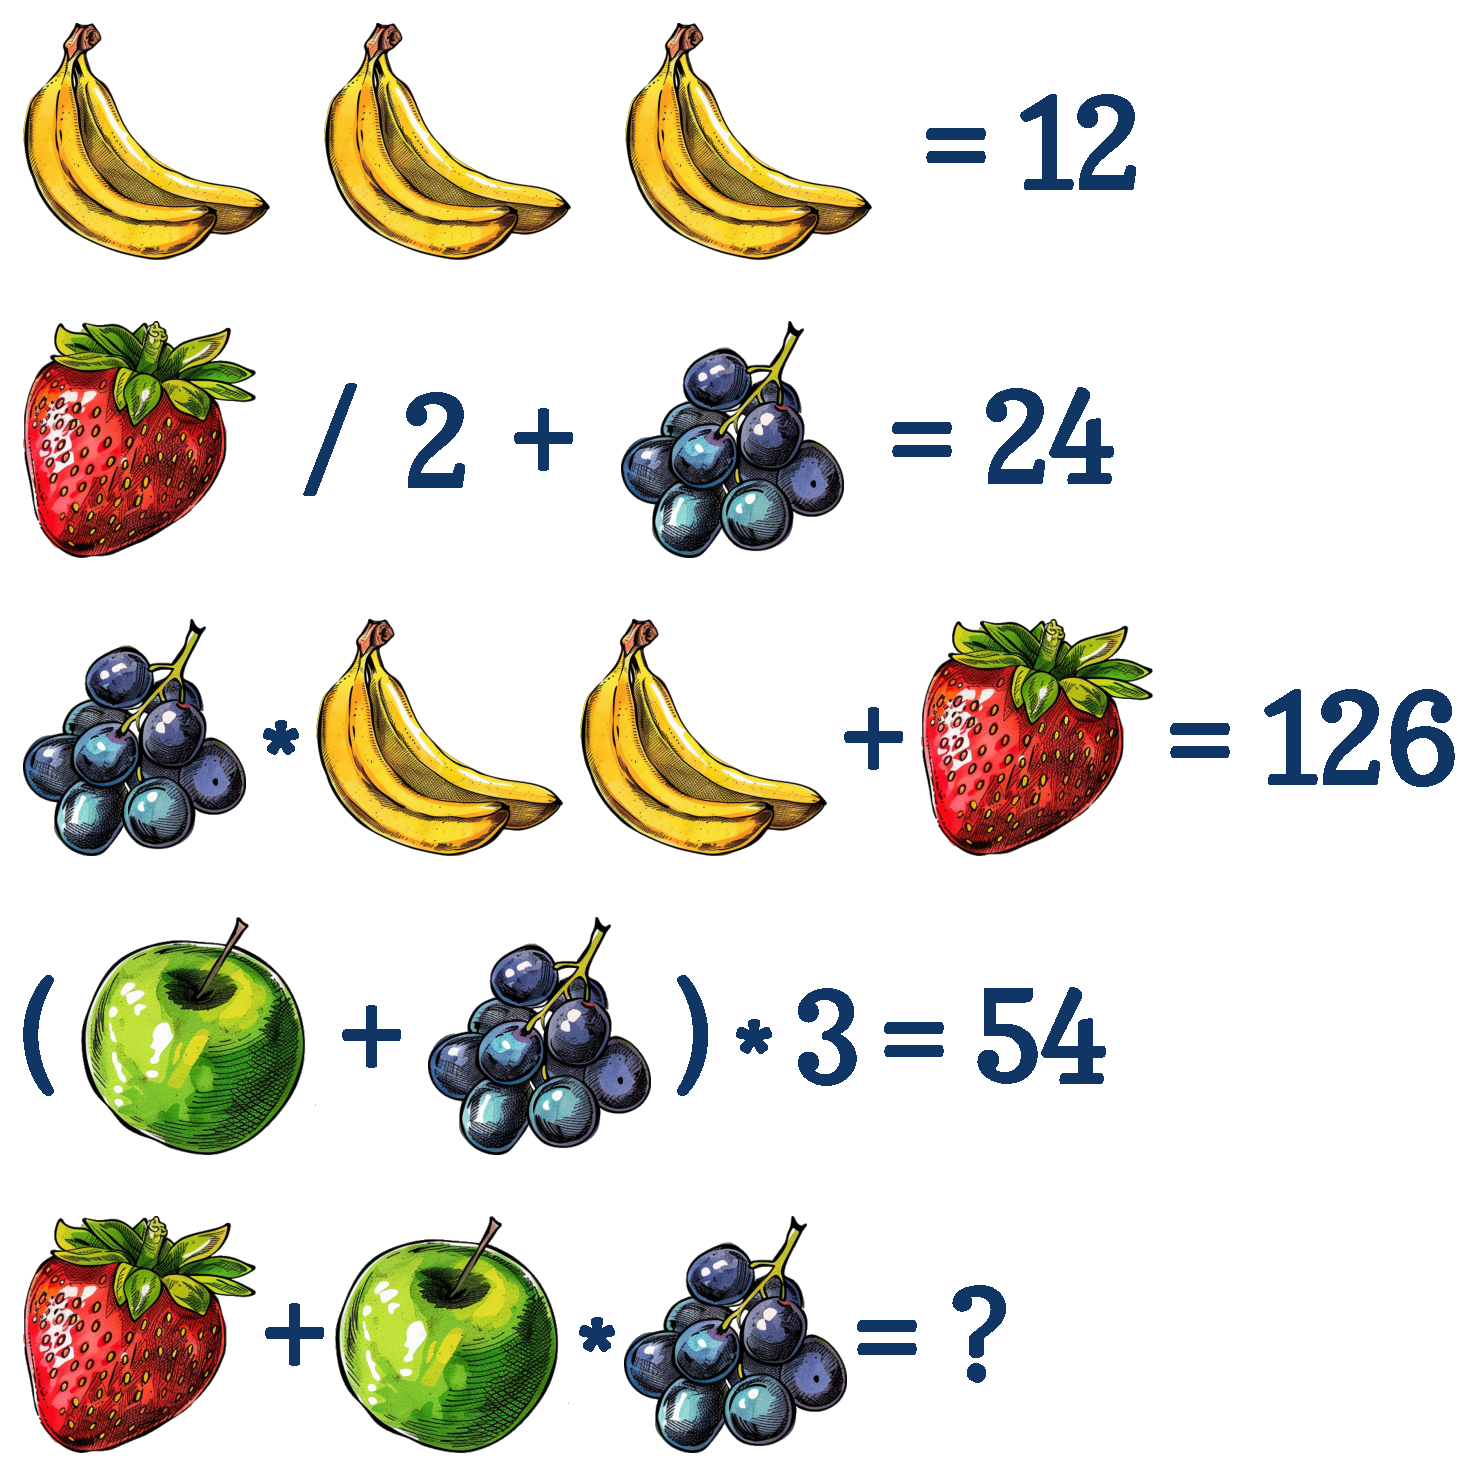
\includegraphics[width=\linewidth]{01equations.pdf}\\
	\end{center}
	
	% 2 bananas  = x
	% strawberry = y
	% grapes = z
	% apple = w
	%
	% x + x + x = 12
	% so x = 4
	%
	% y / 2 + z = 24
	%
	% z * (x + x) + y = 126
	% so 8z + y = 126
	% hence 6z = 78 => z = 13
	% finally, y/2 = 11 => y = 22
	%
	% ( w + z ) * 3 = 54 => w + z = 18 => w = 5
	%
	% y + w * z = 22 + 5 * 13 = 22 + 65 = 87
	
\end{document}